In this chapter, the details of approaches will be discussed. It starts with an overview of local interpretation methods and several variants of them are introduced respectively. Firstly, we present the binary feature flip idea which aims to characterize the impact of binary features by flipping the feature values. After that, we are interested in the effect of numeric features in the model by inspecting the outcome change of the model when the numeric feature values are perturbed to generate noises. Despite the "variable-specific" methods, we also focus on local interpretable model-agnostic explanations (LIME) which is able to explain individual predictions for any types of features and models. However, no theory can support why LIME can fit linear behavior locally on black box models. Therefore, we continue exploring Shapley value, which is a reasonable explanation method with well-founded theory. In addition, the appealing approach assigns a contribution score for each feature value to smooth the path of interpreting the final prediction of individual instances by calculating the Shapley value. 

Then the following section describes the novel technique which combines the local interpretation methods and pattern mining technique. Since the target concept during subgroup discovery in our situation is either prediction change or feature influence score, therefore, the focus shall attribute to numeric target. Later, the standard approaches to measure the interestingness of subgroups are discussed. Furthermore, methods to avoid redundancy in subgroups are explored. 

%Text classification or document classification is one of the most important tasks in Natural Language Processing field. Its primary goal is predicting the label or a class of a given document based on words, characters or other available features. Text classification has been extensively studied, and it has been used in a various application, the most famous one would be detecting spam letters in email clients
\subsection{Structure of interpretation framework}

As you probably have noticed that the adoption of complex machine learning models which have high performance is growing rapidly. Driven by the boosting awareness of machine learning field, the urgent need to interpret those complicated black box models is occurred. Besides, external pressures are withstood by the enforcement of regulations like GDPR in EU. Given the situation, the research about interpretable machine learning are quite active. 

Generally, many existing approaches for interpreting black box models are based on the model prediction, i.e., generating an explanation for the model prediction by inspecting the variable influence from the input, which is operated on the instance level. Concluded by Alvarez-Melis \cite{alvarez2018robustness}, those methods can be roughly categorized as salience-based and perturbation-based approaches. The former method category is also known as gradient-based attribution methods, computing the partial derivatives of the output with respect the each input feature, e.g. Integrated Gradients \cite{selvaraju2017grad}\cite{sundararajan2017axiomatic}. In contrast, perturbation-based approaches first generate a bunch of neighborhood data points surrounding the instance to be explained, then calculate the contribution of each input features towards the output by fitting a local interpretable model, e.g. LIME \cite{ribeiro2016model}.  

With those theoretical methods, a list of machine learning interpretability framework are surfaced. For instance, DeepExplain is a unified framework of perturbation and gradient-based attribution methods for deep neural networks interpretability which can be found in \cite{deepexplain}, referring to the method presented by Marco\cite{ancona2017towards}. Another framework is LIME, which supports explaining the predictions of any machine learning classifiers, founding on the perturbation-based approach. And the framework is available in \cite{lime}. In addition, a promising framework called SHAP could connect the game theory with local explanations to provide understandable interpretations for any black box models, which is accessible and open sourced on \cite{shap}. 

After seeing these frameworks, it could be easily observed there are huge drawbacks for each single framework. DeepExplain is mainly designed for image classifier that is using deep neural network. Even though LIME is applicable to tabular data, text data, and image data, the framework support for complicated models such as deep neural network is not well implemented. And the the exact evaluation of Shapley values is prohibitively expensive in SHAP framework, which cannot be used as an online algorithm. What is worse, even non of those frameworks include the global interpretation view on the black box models, which is handy in many situations.

In light of those flaws, we aim to construct a new interpretation framework. From a large point of view, the global interpretation methods and local interpretation methods are included. For a global interpretation, feature importance ranking is supported by the permutation feature importance method. On the other hand, the existing local interpretation methods like LIME and SHAP are incorporated into the new framework. Besides, two very simple model-agnostic approaches, named as binary feature value flip and numeric feature value perturbation respectively, are implemented as well. Nevertheless, the most important contribution is that we manage to derive a mid-level interpretation of black models between global interpretation view and local interpretation view by combining the local interpretation methods and subgroup discovery technique. In this way, we are supposed to discover interesting patterns in dataset where the inspected variable impose large impact. 

In the following, two large components in the framework will be introduced separately, which are local interpretation methods and subgroup discovery technique. 

%TO DO: provide more concrete examples
\subsection{Local interpretation methods}

In comparison to Global interpretable methods which are dedicated to explain the global model output by comprehending the entire datasets, it is more interesting to examine the model prediction for an individual instance. Besides, it could be observed that the global interpretation methods are less sensitive to noises if we make some perturbations on feature values, however, it could lead to tremendous changes in the prediction for an instance. Therefore, the local explanations shall preserve high accuracy than global explanations. In the following, few local interpretation methods will be covered in detail. 

\subsubsection{Binary feature value flip}

Binary feature implies that the feature only contains two unique values. In another word, if it is encoded as discrete numeric number, the feature value should be either 1 or 0. Thus, to flip binary feature value means to convert from 1 to 0 or the other way around. In practice, we could also use the XOR operation to map from 1 to 0. For instance, gender is regarded as a binary feature which only holds value "male" and "female". 

As mentioned previously, the assumption is that we hold the dataset and the corresponding model trained on that dataset. Initially, we could obtain the prediction from the model for a specific instance. Then, a binary value is flipped on a chosen feature and afterwards a new prediction is generated by applying the model to the modified instance. Therefore, as a simple measurement, the effect of this binary feature could be estimated by the difference between two outputs. 

In practice, there are two variants to assess the variable influence. One way is to calculate the absolute difference of two predictions, and in this way we could ignore the bias of this binary feature on the original dataset. Literally to say, the binary feature is more influential when the difference becomes larger. In contrast, we could compute the difference for a defined direction, for example, we just care about the effect of gender changing from male to female. In this case, not only the magnitude of the effect is obtained, but also the positive or negative sign towards the prediction.  

\subsubsection{Numeric feature value perturbation}

As the name suggests, this technique is applicable to features whose type is numeric. The idea is that we could apply binary operations to the input values to produce new values, which serves as injecting noises into the original dataset. In particular, only addition and subtraction are considered in this situation. For example, an instance includes a numeric feature called "age" and we could perturb this feature value by increasing or decreasing by a certain value to obtain the modified value. 

The procedure of measuring the effect of a chosen input feature is similar to that in binary feature value flip approach. For classification or regression tasks, we could make predictions with the existing model on the instance we desire to explain. Afterwards, a new prediction is made on the adapted instance which is produced through perturbation on the selected numeric feature. And the impact of this numeric feature could be approximately evaluated by the absolute difference of two output predictions, which indicates that this particular feature plays an important role in this instance, causing unstable predictions. Roughly to say, larger prediction differences might imply the feature has a stronger effect on the corresponding instance. 


\subsubsection{LIME: Local Surrogate}

Various criteria can be used to classify types for machine learning interpretability. Intrinsic interpretability, for example, is one type of the interpretability methods, which refers to models that are intrinsic interpretable owing to their simple structures, such as linear models or decision trees. In contrast, post hoc interpretability is meant to analyze the model interpretability after model training. As introduced earlier, permutation feature importance is a post hoc interpretation method. 

In this thesis, we would like to focus on post hoc interpretability, which indicates to explain model decisions after the model has been trained. In particular, model agnostic interpretation methods, which extracts post hoc explanations by treating the original model as a black box, is highly valued. The model agnostic interpretation method is pretty flexible in terms of models, and it can work with any type of machine learning models, which provides a great advantage over model-specific methods \cite{ribeiro2016model}. The principle behind is to learn an interpretable model on the decisions of the black box model and in return apply the interpretable model to those predictions that are expected to explain.  

Following this idea, it leads us to the local surrogate methods, which are able to explain individual predictions of any black box models in a faithful way. As a concrete implementation of local surrogate models, Local interpretable model-agnostic explanations (LIME) was initially proposed in paper \cite{ribeiro2016should}. 
%It might be noticed that the previously presented approaches are constrained within a certain situation and the stability or accuracy is not guaranteed either. Naturally, the aim comes to discover approaches to explain individual predictions of any black box models faithfully, leading us to the local surrogate methods. As a concrete implementation of local surrogate models, Local interpretable model-agnostic explanations (LIME) was initially proposed in paper \cite{ribeiro2016should}. 

The key point behind LIME is pretty straightforward. It is intended to explain individual explanations by fitting a simple interpretable model to locally approximate the underlying black box model. The typical choice of the interpretable model could be regularized linear models like Lasso or decision trees. To elaborate more intuition for LIME, the toy example is shown in \ref{fig:lime}. This is a binary classification task and the regions colored with blue or pink are regarded as two distinct decisions. Evidently, this decision function can not be easily interpreted by a linear model. As a clarification, we are interested in the individual instance explanation, which is marked with a bold red cross. To fit a local interpretable model, some artificial points are created by perturbing the original data point. The learned local model, marked by the dashed line, could in principle provide a faithful explanation for the target instance. 

\begin{figure}[H]% use[!htb] to force the latex ignore the defaut
	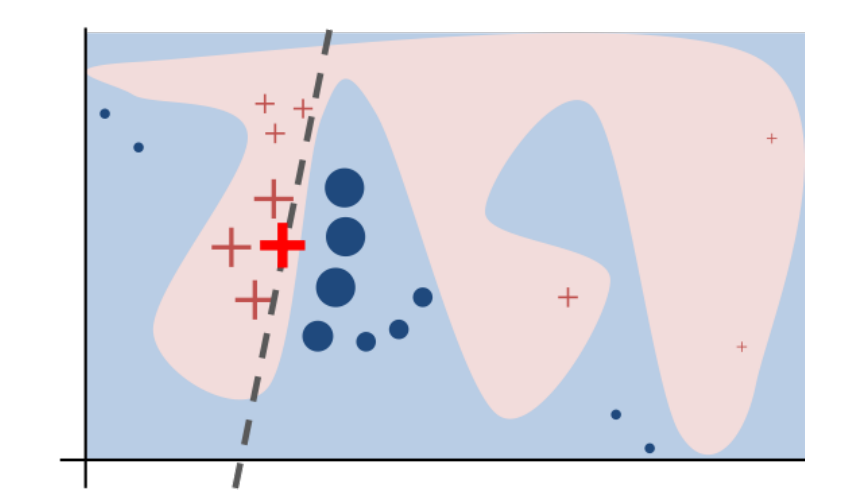
\includegraphics[width=0.9\textwidth]{imgs/lime.png}
	\caption{Binary classification task for a black box model. Decision regions are colored with a blue or pink background. Instance to be explained are marked in a bold red cross. Artificial points, marked as crosses and circles, are created by perturbing the instance of interest, whose size are weighted by the proximity to the instance. The dashed line expresses the fitted local interpretable model which could give faithful explanations.}
	\label{fig:lime}
\end{figure}

Apart from the intuition, we could argue for the faithfulness from a mathematical perspective and the constraint of LIME could be represented as equation \ref{eq:lime}. 

\begin{equation} \label{eq:lime}
\begin{gathered}
\xi=\underset{g \in {G}}{\arg \min } L\left(f, g, \pi_{x}\right)+\Omega(g)
\end{gathered}
\end{equation}

As formally defined in the equation, f is the black box model, g is the local explanation model needs to be figured out, and G is a group of interpretable models, which includes linear models, decision trees, or falling rule lists \cite{wang2015falling}. As depicted in the figure, the weight is measured by the proximity of instance of interest to the surrounding artificial instances, which is defined as $\pi_{x}(z)$. And the complexity of explanation model g is described as $\Omega(g)$. For example, the complexity could be estimated by the depth of trees for decision trees models or by constraining the maximum number of features in linear models. Thus, as seen from the formula, in order to obtain the local explanation model for instance x, the loss L (e.g. mean squared error) should be minimized while maintaining the complexity as low as possible.

In practice, the general procedure to train an explanation model is described as follows: First, select an individual instance that we desire to explain for its black box prediction. Then, generate artificial data points by perturbing the selected sample and make predictions for these new instances using the original model. Afterwards, calculate the weights for new instances according to their proximity to the instance being explained. Next, fit a weighted, interpretable model on the obtained dataset. Finally, interpret the instance prediction by utilizing the trained local interpretable model. 

After a literature review, it is found that LIME is one of the few methods that work for tabular data, text and images, which is a very promising approach. The python implementation is currently available in \cite{lime}, which is still in active development and needs further exploring. 

\subsubsection{Shapley values}
%In response to this we chose to use a model agnostic representation of feature
%importance, where the impact of each feature on the model is represented using Shapley values
%comparing model output using all of the permutations of variables to try and derive the impact of each individual variable

As we have seen, numerous approaches have been recently proposed to explain predictions for individual instances of black box models. As stated in \cite{robnik2008explaining}, the presented approach is relied on the decomposition of a prediction for a single instance on individual contributions of each attribute, and the contribution for each feature value is measured as the difference between the output value and the average output over all perturbations of the corresponding feature. Nevertheless, this approach fails to work if the features are conditionally dependent. 

Inspired by the coalitional game theory which instructs us to fairly distribute the "payout" among the "players", a general method for explaining black box models by taking into account interactions between features can be found in \cite{kononenko2010efficient}, whose fundamental concepts are borrowed to explain instance-level predictions with contributions of each feature values. Corresponding to the known concept in coalitional game theory, the contributions of individual feature values are called Shapley Value.

Despite from the abstract concept, an illustration taken from \cite{molnar2019} might help us intuitively understand the Shapley value. Imagine there is a room and all feature values of an individual instance enter the room in a random order. All feature values, seen as players, need to collaborate with each other to participate the game, where each player contributes to receive the final prediction. And each order of feature values represents a coalition. Consequently, the Shapley value of a feature value corresponds to a difference in the value of a coalition when the feature is added to it. In other words, the Shapley value is the average marginal contribution of a feature value across all possible coalitions. 

Then, let us have a detailed look at the formal definition of Shapley value as expressed in equation \ref{eq:shapley}, where S is the subset of the features in an individual instance, p is the number of features, and x is the vector of feature values of the instance to be interpreted. As for characteristic function val, it describes the contribution of feature j in each coalition.


%The best explanation of a simple model is the model itself; it perfectly represents itself and is easy to understand. For complex models, such as ensemble methods or deep networks, we cannot use the original model as its own best explanation because it is not easy to understand. Instead, we must use a simpler explanation model, which we define as any interpretable approximation of the original model


\begin{equation} \label{eq:shapley}
\phi_{j}(v a l)=\sum_{S \subseteq\left\{x_{1}, \ldots, x_{p}\right\} \backslash\left\{x_{j}\right\}} \frac{|S| !(p-|S|-1) !}{p !}\left(\operatorname{val}\left(S \cup\left\{x_{j}\right\}\right)-\operatorname{val}(S)\right)
\end{equation}

Referred to \cite{shapley1953value}, the Shapley value can provide the unique solution that adheres to he desirable properties, which are Efficiency, Symmetry, Dummy, and Additivity.

\textbf{Efficiency}: denoted as \ref*{eq:efficiency}, which requires that the sum of feature contributions must equal to the difference of the final prediction and the average prediction over all coalitions. 

\begin{equation} \label{eq:efficiency}
\sum_{j=1}^{p} \phi_{j}=\hat{f}(x)-E_{X}(\hat{f}(X))
\end{equation}

\textbf{Symmetry}: The contributions of two feature values j and k are the same, which means equation \ref{eq:symmetry} should be satisfied. 

\begin{equation} \label{eq:symmetry}
\begin{gathered}
\begin{aligned}
if \ val\left(S \cup\left\{x_{j}\right\}\right) &= val\left(S \cup\left\{x_{k}\right\}\right) \\
then \  \phi_{j} &= \phi_{k}
\end{aligned}
\end{gathered}
\end{equation}

\textbf{Dummy}: The contribution of feature j is 0 if it does not change the predictions when it joins into any coalitions. This properties can be demonstrated in equation \ref{eq:dummy}.

\begin{equation} \label{eq:dummy}
\begin{gathered}
\begin{aligned}
if \ val\left(S \cup\left\{x_{j}\right\}\right) &= val\left(S \right) \\
then \  \phi_{j} &= 0
\end{aligned}
\end{gathered}
\end{equation}

\textbf{Additivity}: For any pair of games v, w, the combined payouts should equal to the sum of two individual payouts, as shown in equation \ref{eq:additivity}. For example, if we trained a random forest and the additivity axiom guarantees that we can calculate the Shapley value for each tree respectively then average them to obtain the final Shapley value. 

\begin{equation} \label{eq:additivity}
\begin{gathered}
\begin{aligned}
\phi_{j}(v+w) &= \phi_{j}(v) + \phi_{j}(w) \\
where \ (v+w)(S) &= v(S) + w(S)
\end{aligned}
\end{gathered}
\end{equation}

\subsection{Kernel SHAP}
%In addition to the aforementioned LIME and SHAP
%Unfortunately, the exact evaluation of Shapley values is prohibitively expensive, exponential in the number of input features. In this work, by leveraging recent results on uncertainty propagation, we propose a novel, polynomial-time approximation of Shapley values in deep neural networks. We show that our method produces significantly better approximations of Shapley values than existing state-of-the-art attribution methods (Explaining Deep Neural Networks with a Polynomial Time Algorithm for Shapley Values Approximation)

Though classical Shapley value leads to a potentially promising result, this approach is too computationally expensive owing to computations for the exponential number of possible coalitions. Feasibly, approximation algorithms could be used to reduce the computational complexity, nevertheless, it inevitably will increase the variance for the calculation of Shapley value. What is worse, the explanation for the prediction of a model is just a simple value, rather than an explanation model like LIME, which fails to make judgments about the connections between input change and prediction change. To address those problems, Lundberg and Lee \cite{lundberg2017unified} proposed a unified framework for explaining predictions, which is based on the Shapley value, and they named it SHAP(SHapley Additive exPlanations). This novel approach unifies existing explanation methods and brings more clarity to the methods space. They introduced the explanation model by treating the explanation of an individual prediction as a model. Of course, the unique solution is guaranteed with the game theory. In addition, it provides a more human-understandable and intuitive explanation by user studies as they claimed. 

In this case, SHAP values are introduced as a novel measure of feature contribution. Similar to classical Shapley value estimation methods, SHAP values provide the unique additive feature importance measure if the flowing properties are satisfied, which are Local accuracy, Missingness, and Consistency \cite{lundberg2017unified}. From another perspective, SHAP method transforms the Shapley value approach into an optimization problem by using kernel function to measure proximity of instances. Within this domain, the novel approximation model agnostic method is called kernel SHAP, which is a combination of LIME and Shapley value. In order to use linear explanation model to locally approximate predictions, we should minimize the following objective function \ref{eq:lime}. 

It is intended to obtain the unique solution of equation \ref{eq:lime}, which should also be in line with those three properties, the Shapley kernel is defined as \cite{lundberg2017unified}:

\begin{equation} \label{eq:shap_kernel}
\begin{gathered}
\begin{aligned} \Omega(g) &=0 \\ \pi_{x^{\prime}}\left(z^{\prime}\right) &=\frac{(M-1)}{\left(M \text { choose }\left|z^{\prime}\right|\right)\left|z^{\prime}\right|\left(M-\left|z^{\prime}\right|\right)} \\ L\left(f, g, \pi_{x^{\prime}}\right) &=\sum_{z^{\prime} \in Z}\left[f\left(h_{x}\left(z^{\prime}\right)\right)-g\left(z^{\prime}\right)\right]^{2} \pi_{x^{\prime}}\left(z^{\prime}\right) \end{aligned}
\end{gathered}
\end{equation}
where $|z^\prime|$ is the number of non-zero elements in $z^\prime$

The SHAP framework recently is in active development and is accessible at \cite{shap}. Since it is seemed to be a very optimistic approach and we are quite interested in this novel model explanation method, therefore, further experiments will be conducted. 


\subsection{Pattern mining with Local interpretation methods}

It appears from the aforementioned sections that a bunch of local interpretation methods which could be exploited to explain an individual black box model prediction were incorporated into our interpretation framework. Attempts were made to investigated those local interpretation methods. In principle, it was assumed that we could obtain a local explanation model for each model prediction independent from the underlying black box model. To put it another words, the instance-level explanation for a chosen prediction shall remain consistent even though the underlying black box model was modified. Nevertheless, situations could happen that two disparate explanations were provided for the same instance prediction when two different underlying black box models were applied. This unexpected results may be attributed to the excessive interpretation of the selected instance, which was merely one sample instance rather than a representative of all instances. Moreover, insights extracted from an individual instance might be too specific to train a well-fitted explanation model, causing unstable and unreliable explanations. 

Recall from previous part, global interpretation methods and local interpretation methods could provide explanations from a global view point and a local view point on the dataset, respectively. Therefore, to overcome the drawbacks from the global view or local view, we would naturally consider to interpret the black box model from somewhere between the global view and the local view. Inspiration from the idea that black box models could detect hidden patterns in a dataset such that they could exhibit a good performance when executing classification tasks, it came to our mind pattern mining was exactly the technique could be utilized to discover hidden patterns in a dataset, which coincided with each other somehow. Therefore, a novel method by combining the local interpretation methods and pattern mining technique was proposed in this thesis. In this regard, it was presumed that the novel approach could provide a "pattern level" view point on the dataset. 

To be frankly, it brings more clarity if we discuss these two individual components separately, which also correspond to two techniques. Since we have already covered the discussion about local interpretation methods, it is intended to elaborate the subgroup discovery technique in the following section.  

\subsubsection{Overview of subgroup discovery}

Note that the terminology pattern mining, whose interchangeable name is subgroup discovery, refers to a data mining technique which pursues to find subgroups of data instances that exhibit interesting characteristics with respect to a predefined target variable \cite{herrera2011overview}. Moreover, subgroup discovery is a descriptive technique, which describes enough details such that the results are understandable by human experts.

In a more formal definition, four elements could be considered the fundamental components to compose the subgroup discovery task, which is defined by a quadruple (D, $\Sigma$, T, Q). These elements are illustrated as below \cite{atzmueller2004towards} \cite{lemmerich2014novel}: 

\begin{itemize}
	\item D is a dataset and is formed by a set of instances, and each instance consists of a set of attributes
	\item $\Sigma$ constrains the search space, which is made up of subgroup descriptions (patterns). And patterns consist of a set of selection expressions, also known as selectors.
	\item T represents the target variable for the discovery task. Various types of target concept could be identified, including binary target, numeric target, or complex target. 
	\item Q defines the quality measure criteria. Different quality measure criteria are specified for different types of target concept. 
\end{itemize}

In principle, the dataset could be any kind of data type, nevertheless, we will primarily concentrate on tabular data, textual data, and sequence data. Actually, the detailed description about the datasets that are used in this thesis will be discussed in the next section, and thereby it will not be deeply investigated here. As for the search space, commonly it is accepted as conjunctive combinations of selectors for the reason that such subgroup descriptions are interpretable by practitioners. As an example, a pattern could be formatted as: $P = sel_1 \wedge sel_2 \wedge ... \wedge sel_d$, where all selection expressions are evaluated to be true. Loosely speaking, the full search space is exponential to the number of input features of the dataset, which can significantly affect the pattern mining efficiency. By taking the size of the search space into account, beam search strategy is adopted to shrink the search space in order to speed up the subgroup discovery task and more detailed information will be illustrated later. 

The choice of the target concept is normally task driven and closely related to the dataset. Using a binary variable as the target of subgroup discovery is a more simple and general situation. Since the binary variable only contains two values (True or False), it is aimed to identify interesting subgroups for each of the possible value. Basically, the idea is to discover patterns whose target share is either remarkably high or remarkably low. However, in this thesis domain, it is desired the discover subgroups which reveals a significant effect of the inspected variable, meaning that the influence scores of the selected attribute are considered as the target concept, which belong to the numeric data type. Generally, pattern mining for numeric target is more complicated because the attribute values could be handled by a numerous approaches such as numeric target discretization in a predefined number of intervals, or dividing the numeric domain into two ranges with respect to the average. And frequently mentioned discretization methods includes equal-width discretization, equal-frequency discretization, and etc. An overview of discretization methods for a numeric attribute was reported by Garcia et al. \cite{garcia2012survey}. In this thesis, it is more inclined to apply the equal-frequency discretization method. 

Without any doubt, it is critical to choose the quality measure carefully, since the results of subgroup discovery are mostly controlled by the quality measure criteria. In light of the fact that the interestingness measure plays a decisive role in the subgroup discovery task, thus, a comprehensive discussion about quality measure for numeric target will be presented in the following subsection.

\subsection{Interestingness measure for numeric target}

% 
% The probably most applied of these measures are the generic mean functions since they are adaptable in iterative approaches and easy to explain to humans with little mathematical expertise.
% In contrast, using the distribution of the numeric targets concept directly with a mean-based interestingness measure, a subgroup is described like “While in the general population the mean age is 56 years, in the subgroup described by xy it is 62”

As was said before, the interestingness measure for numeric target becomes more complex to investigate than situations where binary values was chosen as the target. Nevertheless, a list of interestingness measures for numeric target was reviewed by Pieters et al. \cite{pieters2010subgroup}. As could be summarized, those interestingness measures were heavily relied on the basis of the statistical distribution of numeric values, such as mean value, median value, or variance. And the general idea behind was to design the interestingness measure for numeric target with respect to those predefined data statistics. More specific, interesting subgroups would be discovered if the computed data characteristic in the subgroup was significantly deviating from the value calculated in the entire population. Referred to paper \cite{lemmerich2014novel}, five categories of interestingness measure for numeric target were outlined, which included mean-based measures, median-based measures, variance-based measures, distribution-based measures, and rank-based measures. Since the mean-based measure was widely accepted and applied in many applications, therefore, it was selected as the primary quality measure for numeric target in later experiments. 

In point of fact, within this mean-based measure family, several concrete interestingness measures could be further explored, distinguishing by the evaluation functions. Take an example, one simple evaluation function could be \textit{Average function}, which calculated the difference between the mean value in the subgroup and the mean value in the entire dataset, denoted as: $q_{mean} = \mu_p - \mu_{\emptyset}$. However, subgroup size was not considered in the former measure, which might be too fragile in certain circumstances. Actually, it was often observed from literature that \textit{Generic mean function} was the most prevalent mean-based interestingness measure due to its simplicity to be interpreted. And the general formulation is denoted in Eq. \ref{eq:mean_based}, where $i_{P}$ was the size of the subgroup, $a$ was a parameter which weighted the subgroup size and deviations, and $\mu_{P}, \mu_{\emptyset}$ represented the average value in the subgroup and the average value in the dataset, respectively. In particular, the choice of parameter $a$ could be selected in an iterative process. For example, $a$ was required increment if the subgroup size was too small to have a significant score, meanwhile, low parameter values for $a$ was preferred with a high deviation of mean target values between the subgroup and the overall dataset. Therefore, after calculating the interestingness score for each subset, those subgroups with significantly higher or lower mean values were considered as interesting and the descriptions of them were our desirable interesting patterns. 

\begin{equation}  \label{eq:mean_based}
q_{mean}^{a}(P)=i_{P}^{a} \cdot\left(\mu_{P}-\mu_{\emptyset}\right), a \in[0,1]
\end{equation}


\subsection{Algorithms}
Apart from the quality measure, the search strategy is critical since the dimension of the search space and time complexity if of great concern. Various strategies could be used, e.g. exhaustive methods, seeking to acquire the optimal subgroup by traversing through the whole search space. In contrast, heuristic approaches, normally a beam search strategy \cite{clark1989cn2}, is often used for subgroup discovery due to its efficiency, which aims to find interesting patterns but not necessarily the optimal patterns in a short time. The intuition behind is that it is assumed that the patterns are more likely to be interesting if their generalizations are also interesting. Therefore, the search starts with an empty hypothesis, then it tries to find the best patterns with size k (corresponding to beam width) by evaluating all selectors in the subgroup discovery task. Following that, at each search iteration, the hypotheses contained in the beam are expanded but only the currently best w hypotheses are kept using a hill-climbing greedy search \cite{atzmueller2015subgroup}. 

\subsection{Redundancy avoidance}

% In particular for numeric target concepts, a comprehensive overview on interestingness measures is provided. Afterwards, two more specific issues for determining interesting subgroups are investigated: The incorporation of generalizations into the assessment of subgroups and the problem of redundant discoveries.
% In many cases, this causes the result set to contain similar, strongly overlapping subgroups, that is, subgroups that cover (almost) the same instances. Since those subgroups are potentially caused by a single phenomenon, presenting multiple overlapping subgroups may provide only little additional information to the user. 

Though patterns could be discovered through the traditional interestingness measure presented above, the results are not ideal, which contains too many redundant patterns. In the quality measure, only the subgroup size and statistics difference between subgroups and entire dataset are considered, which might produce uninteresting patterns when ignoring the selector expressions of subgroups. For example, assume that the mean contributions of age for the entire dataset is at $M_{\emptyset}=0.50$. And the mean value in the subgroup with the expression $age > 40 \cup gender=male$ is $M_{age > 40 \cup gender=male}=0.80$. It seems that the pattern should have a high quality score and is identified as an interesting pattern. However, it is probably not interesting enough if given the information that its generalization has nearly the same value, which means mean value does not deviate significantly from the mean value of its generalizations, e.g. $M_{age > 40} = 0.78$. 

To avoid that such subgroups are included in the result set, Generalization-aware interestingness measures could be applied to improve the traditional selection criteria for pattern mining by considering the statistics of the subgroup and also to its all generalizations. In \cite{grosskreutz2010subgroup}, Grosskreutz et al proposed to estimate the quality of a pattern $P$ as the minimum of the quality of $P$ with respect to the extension of all its generalizations. Denoted as equation \ref{eq:incremental_q}, $q^{\Delta}$ is the incremental version of q, $D$ is the dataset, $P$ is the subgroup and $H$ includes its all generalizations. 

\begin{equation} \label{eq:incremental_q}
q^{\Delta}(D B, P)=\min _{H \subset P} q\left(D B\left[H\right], P\right)
\end{equation}

Since the mean value of the target is mainly explored, the above equation could be formalized in a simpler way, as shown in \ref{eq:generalization_q}. By doing so, redundant patterns are avoided and more interesting subgroups are discovered. 

\begin{equation} \label{eq:generalization_q}
q_{\operatorname{mean}}^{a}(P)=i_{P}^{a} \cdot\left(\mu_{P}-\max _{H \subset P} \mu_{H}\right), a \in[0,1]
\end{equation}

\subsection{Combination with local interpretation methods}

Recall from local interpretation methods, the contribution values for each variable of an individual instance could be obtained by using the explanation model to interpret the black box model. In this case, the contribution score of the chosen variable is our target, which is naturally to be numeric. Now, the next step goes to the traditional pattern mining problem, aiming to discover subgroups of the population that are statistically interesting. 


\subsection{Decision trees with Local interpretation methods}
%In the next section, we completely switch gears.

The Decision Tree is a supervised machine learning method used for classification and regression tasks. It is called "Decision tree" because the structure of each decision tree is a tree-like graph and model is constructed to predict the target by learning simple decision rules inferred from data attributes. Decision tree itself is an interpretable model that can provide human-understandable decisions by exploring the decision rules. To be specific, a decision tree applies a recursive partition technique, which keeps on splitting the data based on the selected attributes. From another perspective, it is also a predictive rule-based approach, which could be used to mine local patterns through the decision path, where each path is traversed from the root node to a leaf node. In literature, numerous methods to create decision trees have been proposed and the main difference between decision tree induction strategies is in their attribute selection methods \cite{quinlan1986induction}. 
(Besides, it is worth to be mentioned that the decision tree finds the optimal splitting pattern by essentially limiting the number of conditions to one. \cite{zimmermann2009cluster})



